The time constant of each detector is a key property that describes the stability and time response of the detector. If the time constant is too large, it must be accounted for in the demodulation of the signal from the HWP polarization modulation, in setting the scanning frequency of the telescope, in measuring the telescope beams and pointing, and in determining the polarization angles of the detectors (if using a HWP). The optical time constant $\tau_{opt}$ is often expressed in terms of the 3dB frequency $f_{3 dB}$, which is given by $f_{3dB}=1/(2\pi \tau_{opt})$. There are several ways to measure the detector time constants.

\paragraph{Planet Scan Method} The time constants of the detectors can be probed by scanning quickly over bright objects such as planets, but our ability to probe such features might be limited by the maximum scan speed of the telescope mount and the low signal to noise on an individual planet scan.

\paragraph{Bias Step Method} The bias step method characterizes the electrical time constant of a detector $\tau_{el}$ by inputing a low amplitude square wave through the bias line and fitting the exponential response. The current $I$ as a function of time $t$ goes as
\begin{equation}
I(t) \propto e^{\frac{\pm t}{\tau_{el}}},
\end{equation}
where the exponential is positive as the voltage is increased and negative as the voltage is decreased. The bias step method is quick and easy to perform before measurements, but $\tau_{el}$ must be properly correlated to optical time constant measurements to determine the optical time constant $\tau_{opt}$.

\paragraph{Amplitude Method} With the amplitude method, the time constants are determined by modulating a source with a chopper at various frequencies and measuring the amplitude of the detector responses with the HWP stationary (if using one). The response in power $P$ of the detectors is given by
\begin{equation}\label{eqn:tc_amp}
P(f) \propto \frac{1}{1+\Big(\frac{f}{f_{3dB}}\Big)^2},
\end{equation}
where $f_{3dB}$ is the optical 3dB frequency and $f$ is the modulation frequency of the source. Figure~\ref{fig:tc_chopper} shows the power versus frequency measurements from two measurements on ABS with their fits.

The optical time constant of a detector increases with increasing loading, and with this method, the added loading from the atmosphere near the horizon behind the source can be large enough to drastically slow the detector time constants and, in some cases, fully saturate the detectors, making them non-responsive. Thus, the time constants measured with this method may not be representative of the time constants under typical loading conditions. For example, in ABS, this method gave $f_{3dB} \sim 30$~Hz versus the actual average across the whole season of 109~Hz. Additionally, the measured amplitudes can be highly sensitive to changes in loading correlated to the weather. Without the use of the HWP, the atmosphere can cause fluctuations in the signals on order of a pW. The power versus frequency plot in the left panel of Figure~\ref{fig:tc_chopper} shows that the fluctuations can be larger than the effect from the time constants.

\begin{figure}[h!]
\centering
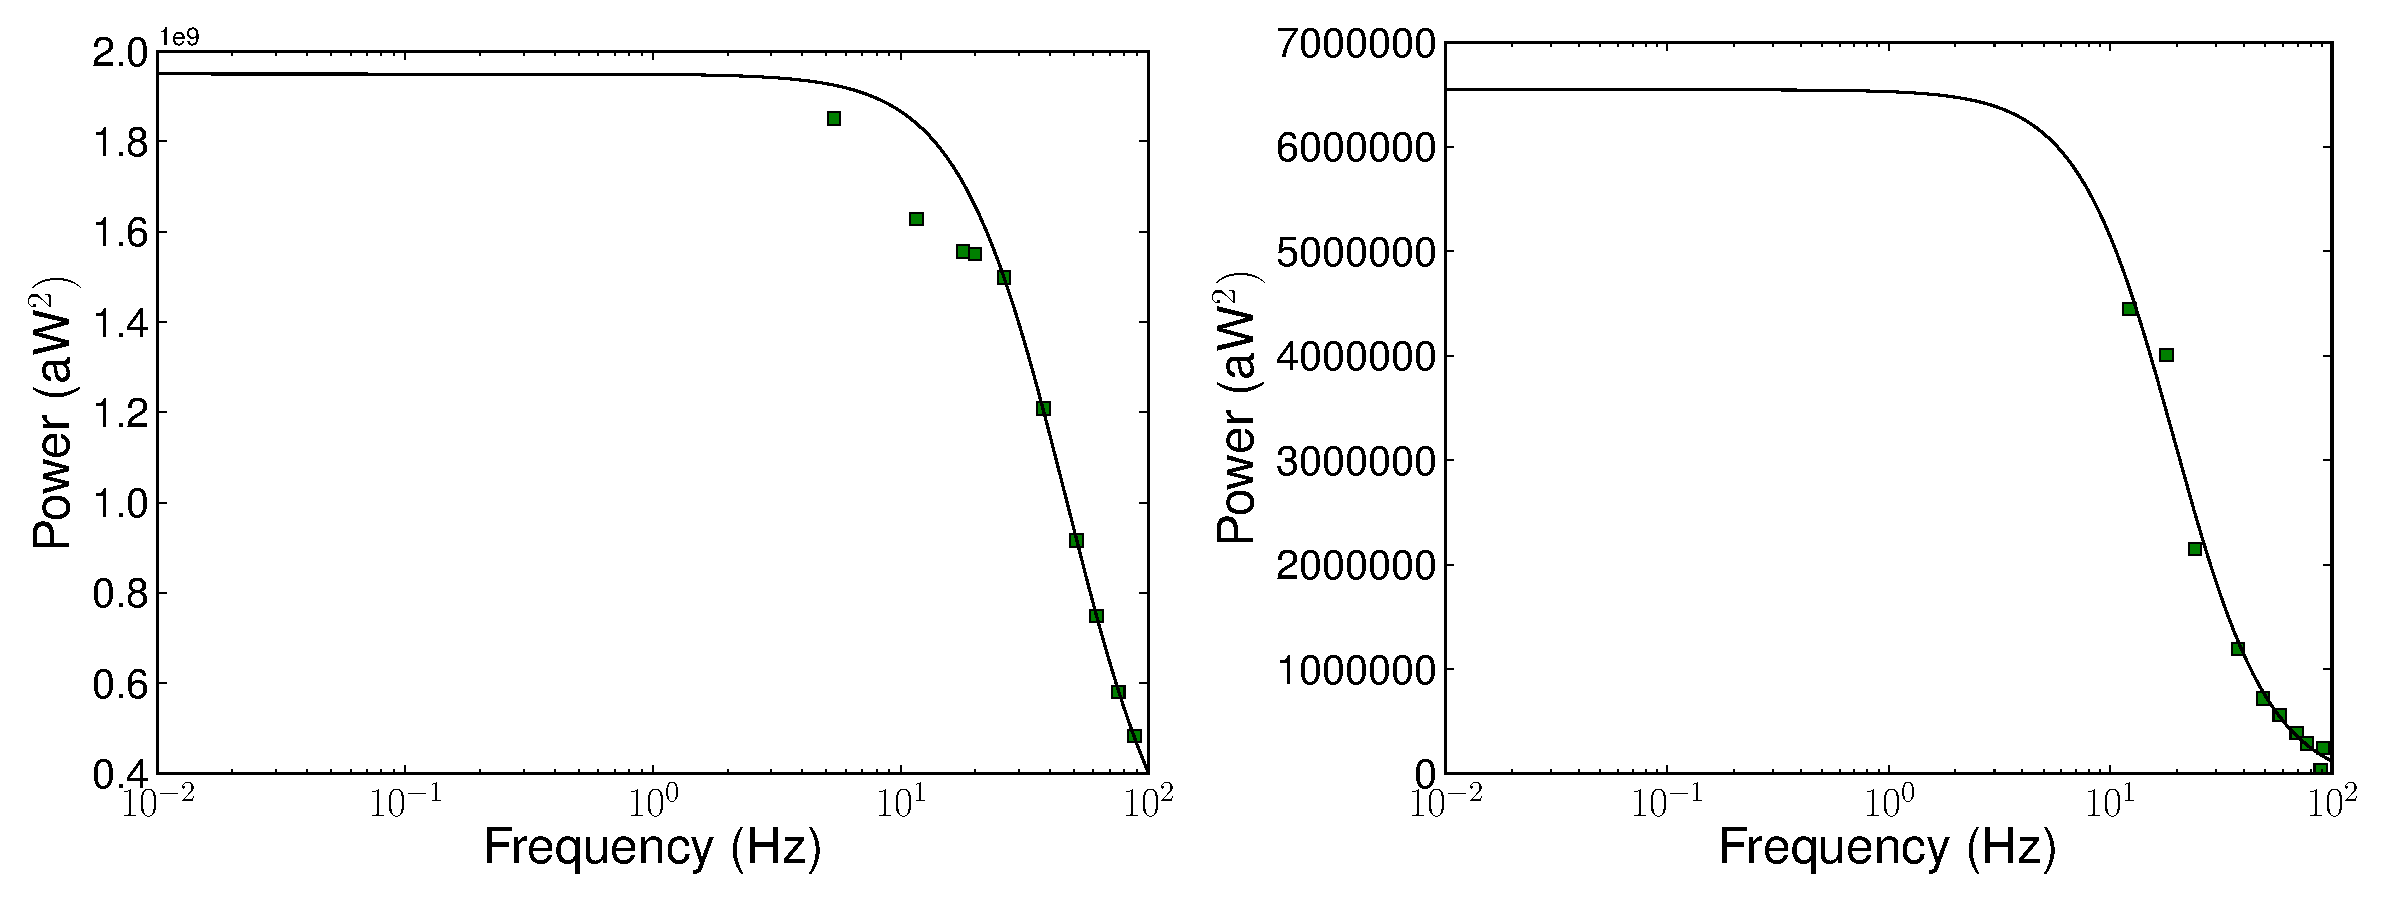
\includegraphics[width=\textwidth]{figures/ampl_pvfreq.pdf}
\caption{The power versus frequency relations are shown above in green with their fits in black for two time constant measurements on ABS. The large atmospheric fluctuations in the first four frequencies of the first measurement and in the last frequency of the second measurement cause the power to fluctuate more than the effect from the time constant, which can be problematic.}
\label{fig:tc_chopper}
\end{figure}

\paragraph{Phase Method} When an experiment has a HWP, the optical time constants can be characterized using the phase delay of the $4f_{m}$ signal~\cite{Simon_LTD2013}. Because it uses the phase, this technique is less susceptible to atmospheric fluctuations over the course of the measurement than the amplitude method. For each phase method measurement, data are taken while slowly varying the rotation speed of the HWP with a sparse polarizing wire grid made positioned above the HWP. The wire grid is used to input a small ($\sim0.1$ pW) polarized signal. This signal adds minimal loading, so the time constants are closer to those during nominal observation. The phase $\phi$ found from demodulating the signal with respect to the polarization modulation frequency $4f_{m}$ is the difference between the physical polarization angle of the grid and the measured polarization angle, which includes the apparent angle rotation due to the time delay of the detector response. It can be modeled as the phase of a one-pole filter: 
\begin{equation}\label{eqn:phi_shift}
\phi=\arctan{\left(\frac{4f_{m}}{f_{3dB}}\right)} + C,
\end{equation}
where $f_{3dB}$ is the optical 3dB frequency of the detector. Because $(4f_{m})^2$ is expected to be much less than $f_{3dB}^2$, the phase can be linearly approximated as 
\begin{equation}
\phi  \approx \phi_0 + \frac{f_{3dB}\,4f_{m}}{f_{3dB}^2+(4f_{m})^2}\approx  \phi_0 + \frac{4f_{m}}{f_{3dB}},
\end{equation}
where $\phi_0$ is a constant offset related to the intrinsic polarization angle of the detector~\cite{Simon_LTD2013}. 
